%%%%%%%%%%%%%%%%%%%%%%%%%%%%%%%%%%%%%%%%%%%%%%%%%%%%%%%%%%
% LMTH 2040 — Calculus: A Multidisciplinary Approach
% Day 01 Handout
% Fall 2026
%%%%%%%%%%%%%%%%%%%%%%%%%%%%%%%%%%%%%%%%%%%%%%%%%%%%%%%%%%

\documentclass[11pt]{article}

\usepackage{../langcalc}

% If langcalc.sty lives in the same directory instead:
% \usepackage{langcalc}

\usepackage{tikz}

\begin{document}

% ========================================================
% PAGE 1 — THE PROBLEM
% ========================================================

\courseheader
    {How Do We Measure an Image?}
    {LMTH 2040 --- Calculus: A Multidisciplinary Approach}
    {August 26, 2026}
    {Eugene Lang College of Liberal Arts}

\vspace{0.5em}

\begin{center}
    \IfFileExists{images/kandinsky8.png}{%
        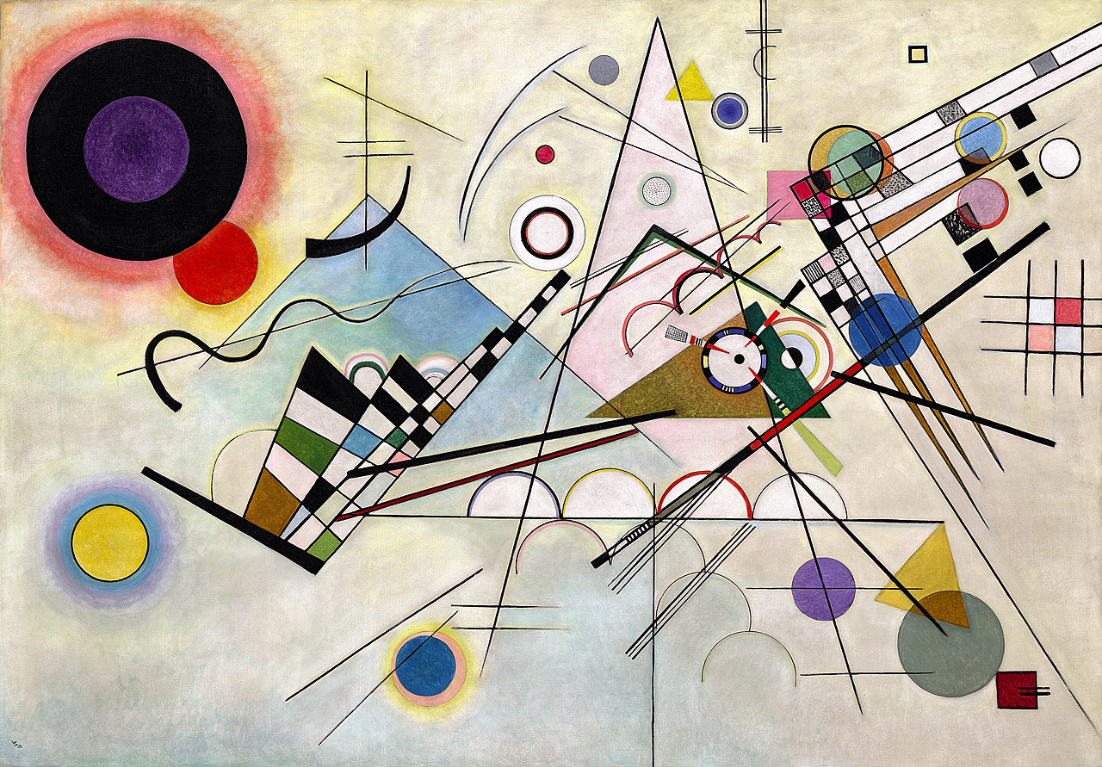
\includegraphics[
            width=\textwidth,
            height=0.56\textheight,
            keepaspectratio
        ]{images/kandinsky8.png}
    }{%
        \fbox{%
            \parbox[c][0.48\textheight][c]{0.9\textwidth}{%
                \centering
                Place \texttt{kandinsky8.png}\\
                in the \texttt{images/} directory.
            }
        }
    }
\end{center}

\vfill

\begin{keyidea}
\centering
\Large
What proportion of this image is occupied by
\textbf{circular forms}?
\end{keyidea}

\vspace{0.75em}

\begin{center}
\large
There is no formula provided.

You may draw on the image, measure it, divide it into pieces,
count things, approximate, or use a calculator.

\medskip

\textbf{Work with your group. Be prepared to explain your method.}
\end{center}

\vfill

\newpage

% ========================================================
% PAGE 2 — FROM MEASUREMENT TO CALCULUS
% ========================================================

\section*{1.\quad Decide what you are measuring}

Before calculating anything, decide what you mean by a
\textbf{circular form}.

What counts? What does not count? How will you treat overlapping,
partially hidden, or outlined forms?

\vspace{1.25in}

\section*{2.\quad Invent a method}

Describe a procedure for estimating the proportion of the image
occupied by circular forms.

Your method should be clear enough that another group could
reproduce it.

\vspace{1.5in}

\section*{3.\quad Make an estimate}

Our estimate is

\[
    \boxed{\hspace{2.5in}}
\]

or approximately

\[
    \boxed{\hspace{1.25in}\%}
\]

of the image.

\section*{4.\quad What could go wrong?}

Identify at least two sources of uncertainty, ambiguity, or error.

\begin{enumerate}[label=\arabic*., leftmargin=2em]
    \item \vspace{0.45in}
    \item \vspace{0.45in}
\end{enumerate}

\newpage

% ========================================================
% PAGE 3 — OPTIONAL / REVEAL AFTER GROUP WORK
% ========================================================

\courseheader
    {Refining the Measurement}
    {LMTH 2040 --- Calculus: A Multidisciplinary Approach}
    {August 26, 2026}
    {Eugene Lang College of Liberal Arts}

\section*{5.\quad Make the method better}

Suppose we place a square grid over the image.

For each square, we decide whether it belongs to the region we
are measuring. This gives an estimate of the proportion of the
whole image occupied by that region.

What happens if we repeat the procedure using increasingly fine grids?

\[
10\times10,
\qquad
100\times100,
\qquad
1000\times1000,
\qquad
\ldots
\]

Let the corresponding estimates be

\[
A_{10},
\qquad
A_{100},
\qquad
A_{1000},
\qquad
\ldots
\]

\begin{problem}
What do you expect this sequence of estimates to do as the grid
becomes finer?

\vspace{1.0in}
\end{problem}

\begin{problem}
Could this procedure eventually produce an \emph{exact} answer?

Why or why not?

\vspace{1.0in}
\end{problem}

\section*{6.\quad A different question}

A computer can calculate

\[
A_{10},
\quad
A_{100},
\quad
A_{1000},
\quad
A_{10000},
\quad \ldots
\]

but it cannot literally complete infinitely many measurements.

\begin{keyidea}
\centering
Can an infinite mathematical process produce an exact finite answer?
\end{keyidea}

\vspace{1em}

\section*{Before you leave}

Respond briefly to each question.

\textbf{\textcolor{LangRed}{MEASURE}} \quad
What had to be decided before your group could produce a number?

\vspace{0.65in}

\textbf{\textcolor{LangRed}{APPROXIMATE}} \quad
Why might increasingly fine measurements approach something more precise?

\vspace{0.65in}

\textbf{\textcolor{LangRed}{QUESTION}} \quad
Can mathematics describe something that neither you nor a computer
could ever literally finish computing?

\vfill

{\small
\textbf{Image revealed after discussion:}
Wassily Kandinsky, \emph{Composition VIII}, 1923.
Oil on canvas, 140 $\times$ 201 cm.
}

\end{document}